% !TEX root = ../paper.tex

\section{UAV-TAlign-1K and Evaluation Protocol}

\subsection{Dataset Scope}

We package UAV-TAlign-1K as a focused public evaluation subset for real UAV RGB-thermal
registration. The subset contains 15 scenes, 500 RGB-thermal pairs, and 1000 images in total. Each
sample is organized as an RGB image paired with a thermal image captured from the same scene
context, while the dataset as a whole spans practical UAV conditions that go beyond standard
near-same-view multimodal matching. In scope and modality, it is closer to recent RGB-thermal
benchmarks such as
KAIST, FLIR, LLVIP, M3FD, DroneVehicle, VTUAV, LasHeR, and Anti-UAV than to classical
same-sensor image matching setups
\cite{hwang2015kaist,flir2018thermal,jia2021llvip,liu2022tardal,sun2022dronevehicle,zhang2022vtuav,li2022lasher,jiang2023antiuav}.

At the scene level, the subset preserves the factors that make reliability assessment meaningful:
day, night, and low-light capture; grayscale and pseudocolor thermal rendering; and both wide-view
and zoom-view scene families. The packaged formal split includes 7 day scenes, 5 night scenes, and
3 low-light scenes; 8 grayscale-thermal scenes and 7 pseudocolor-thermal scenes; and paired
wide/zoom controls for the substation scene family.

\begin{figure}[t]
\centering
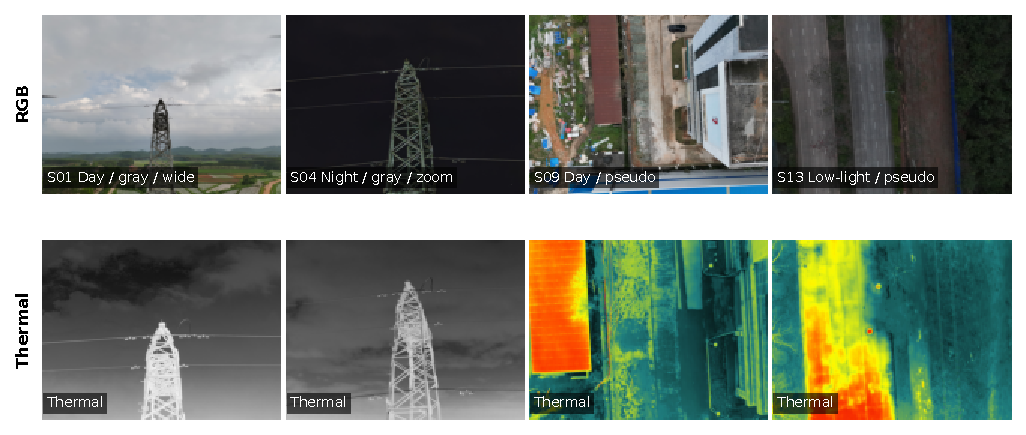
\includegraphics[width=\textwidth]{figures/fig_dataset_examples.pdf}
\caption{Representative UAV-TAlign-1K RGB-thermal pairs spanning day, night, low-light,
grayscale-thermal, pseudocolor-thermal, wide-view, and zoom-view conditions.}
\label{fig:dataset_examples}
\end{figure}

\subsection{Dataset Organization}

Each scene is stored under its own scene directory, and paired samples are formed by matching file
stems between \texttt{rgb/} and \texttt{thermal/} subdirectories. The dataset loader constructs
scene pairs from common RGB and thermal filenames, while scene-level metadata are loaded from the
subset manifest. For each pair, the loader stores scene identity, pair identity, light condition,
thermal rendering, view type, and scene label.

This organization supports both pairwise baseline evaluation and scene-level pipeline evaluation
under the same subset definition, while also enabling condition-based breakdowns from a unified
scene manifest.

\subsection{Complementary Evaluation Units}

The protocol uses two complementary evaluation units. First, off-the-shelf baselines are evaluated
at the pair level. Each of the 500 RGB-thermal pairs is processed independently, and the resulting
statistics describe whether a method can produce a usable pairwise registration and homography
under a fixed off-the-shelf setting.

Second, UAV-TAlign is evaluated at the scene level. Multiple frame-level estimates are aggregated
into a scene-level transform, and the final decision is made by canonical scene acceptance rather
than by pairwise usability alone. The pairwise and scene-level tables therefore provide two
complementary views of practical registration behavior: correspondence availability and retained
scene-level alignment reliability.

\subsection{Label-Free QA Proxies}

The protocol relies on label-free relative QA signals designed for scalable scene-level reliability
analysis. The strongest stored proxies compare the optimized transform against a baseline
initialization and summarize whether scene-level rectification improves cross-modal agreement. The
proxy family includes edge-overlap improvement, gradient-NCC improvement, the ratio of
frames with improved gradient agreement, severe baseline-relative outlier count and ratio,
accepted-frame ratio, and homography-dispersion and robust-rejection diagnostics.

These proxies provide a practical scene-consistency signal for comparing methods and for deciding
whether a scene-level transform is reliable enough to retain, in the spirit of practical
matching-oriented evaluation and benchmarking discussed in prior image-matching literature
\cite{ma2021survey,liao2024survey}.
